\documentclass{beamer}
\usetheme{STCE}

\usepackage{beamerfoils}
\usepackage[utf8]{inputenc}
\usepackage{amsmath}
\usepackage[german]{babel} % Für deutche Umlaute
\usepackage{tabularx} % Für die TabularX Umgebung
\usepackage{listings}

\lstloadlanguages{[ISO]C++}

\lstset{basicstyle=\scriptsize}

\MyLogo{
\centering

\includegraphics[width=0.12\textwidth]{figures/logo.eps}
}

\begin{document}
\title{Korrelation und Regressionsanalyse\\
Finale Präsentation}
\author{Patrick Neidig \and Marius Grysla}
\institute{Software and Tools for Computational Engeneering}
\date{28.06.2011}
\frame{\titlepage}

\begin{frame}
 \frametitle{Inhalt}
 \tableofcontents
\end{frame}

\section{Korrelation}

\subsection{Wiederholung}

\begin{frame}
	\frametitle{Korrelation: Wiederholung}
	
	\begin{block}{Korrelation}
		Zusammenhang zwischen zwei oder mehreren Merkmalen, dessen Stärke sich mit Hilfe von Korrelationskoeffizienten berechnen lässt
	\end{block}
	
	\begin{block}{Bravais-Pearson-Korrelationskoeffizient}
		misst die Stärke des linearen Zusammenhangs zweier mindestens intervallskalierter Merkmale $X$ und $Y$
		
		\begin{equation*}
			r=\dfrac{s_{XY}}{s_Xs_Y}=\dfrac{\sum_{i=1}^{n}{(x_i-\bar{x})(y_i-\bar{y})}}{\sqrt{\sum_{i=1}^{n}{(x_i-\bar{x})^2\sum_{i=1}^{n}{(y_i-\bar{y})^2}}}}
		\end{equation*}
		
		\begin{itemize}
			\item $\bar{x}$/$\bar{y}$: arithmetische Mittelwerte von $X$/$Y$
			\item $s_{X}$/$s_{Y}$: Standardabweichungen von $X$/$Y$
			\item $s_{XY}$: Kovarianz von $X$ und $Y$
		\end{itemize}
	\end{block}
\end{frame}

\begin{frame}
  \frametitle{Korrelation: Berechnung}
	
	\begin{block}{Sukzessive Berechnung}
		\begin{itemize}
			\item arithmetische Mittelwerte (pro Merkmal)
			\item Standardabweichungen (pro Merkmal)
			\item Kovarianzmatrix (für alle Merkmalspaare)
			\item Korrelationsmatrix (für alle Merkmalspaare)
		\end{itemize}
	\end{block}
	
	Interpretation der Ergebnisse:
	
	\begin{itemize}
		\item $r>0$/$r=0$/$r<0$: positive/keine/negative Korrelation
		\item $|r|<0.5$/$|r|\geq0.5$/$|r|\geq0.8$: schwache/mittlere/starke Korrelation
	\end{itemize}
\end{frame}

\begin{frame}
  \frametitle{Korrelation: Ergebnis Mietdatensatz}
  
  \begin{equation*}
		R =
		\begin{footnotesize}
			\begin{pmatrix}
				{\bf 1.00} & 0.47 & {\bf \textcolor{red}{0.71}} & {\bf \textcolor{red}{0.54}} & 0.05 & -0.07 & 0.16 & 0.15\\
   			0.47 & {\bf 1.00} & -0.23 & -0.27 & 0.29 & -0.07 & 0.15 & 0.11\\
  	 		0.71 & -0.23 & {\bf 1.00} & {\bf \textcolor{red}{0.84}} & -0.20 & -0.05 & 0.09 & 0.06\\
	   		0.54 & -0.27 & 0.84 & {\bf 1.00} & -0.15 & 0.03 & 0.00 & 0.03\\
  	 		0.05 &  0.29 & -0.20 & -0.15 & {\bf 1.00} & 0.31 & -0.11 & 0.06\\
  			-0.07 & -0.07 & -0.05 & 0.03 & 0.31 & {\bf 1.00} & -0.31 & 0.06\\
				0.16 &  0.15 & 0.09 & 0.00 & -0.11 & -0.31 & {\bf 1.00} & -0.12\\
  			0.15 &  0.11 & 0.06 & 0.03 & 0.06 & 0.06 & -0.12 & {\bf 1.00}\\
			\end{pmatrix}
		\end{footnotesize}
	\end{equation*}

\end{frame}

\subsection{Planänderungen}

\begin{frame}
  \frametitle{Korrelation: Planänderungen}
	
	Ursprünglich geplant:
	\begin{itemize}
		\item Bravais-Pearson-Korrelationskoeffizient
		\item Rangkorrelationskoeffizienten
		\begin{itemize}
			\item Spearman-Rangkorrelationskoeffizient
			\item Kendall-Rangkorrelationskoeffizient
		\end{itemize}
		\item Partielle Korrelation (optional)
		\item Leistungsanalyse
	\end{itemize}
	
	\pause
	
	Aus Platzgründen (weitgehend) vernachlässigt:
	\begin{itemize}
		\item Kendall-Rangkorrelationskoeffizient
		\item Partielle Korrelation
	\end{itemize}
\end{frame}

\section{Regression}

\subsection{Wiederholung}
\begin{frame}
  \frametitle{Regression: Wiederholung}

  \begin{block}{Regression}
    Bestimmung einer Funktion, die den Zusammenhang zwischen einem Regressanden und einem oder mehreren Regressoren modelliert.
  \end{block}
  
  \pause

  \begin{block}{Multipler linearer Regressionsansatz}
    \begin{equation*}
      Y_i = \beta_0 + \beta_1 x_{i1} + \dots + \beta_p x_{ip} + \epsilon_i, \quad i = 1, \dots, n
    \end{equation*}
    \begin{itemize}
    \item Anzahl der Regressoren: $p$
    \end{itemize}
  \end{block}

  \begin{itemize}
  \item Eine Transformation des Regressanden ist möglich!
  \end{itemize}

\end{frame}

\begin{frame}
  \frametitle{Regression: Berechnung}

  \begin{block}{Methode der kleinsten Quadrate}
    {\centering
      $\sum\limits^{N}_{n=1} \epsilon^2_n = \epsilon^T \epsilon = (y - X \beta)^T (y - X \beta) = $
      $\Vert X\beta - y \Vert_2 \rightarrow \min\limits_{\beta}$
      \\}
  \end{block}
  
  \begin{itemize}
  \item Berechnung mittels QR-Zerlegung von $X$:
    \begin{itemize}
    \item $X = QR^*$, mit $R^* = \binom{R}{0}$
    \item $Q^T * y = \binom{c}{d}$
    \item Löse $R \hat{\beta} = c$ durch Rückwärtseinsetzen
    \end{itemize}
  \end{itemize}

  \pause

  \begin{itemize}
  \item Verfahren zur QR-Zerlegung:
    \begin{itemize}
    \item Householder Transformationen
    \item Givens Rotationen
    \item Modifiziertes Gram-Schmidt Verfahren
    \end{itemize}
  \end{itemize}

\end{frame}

\begin{frame}
  \frametitle{Regression: Ergebnis Mietdatensatz}
  
  \begin{figure}[t]
    \centering
    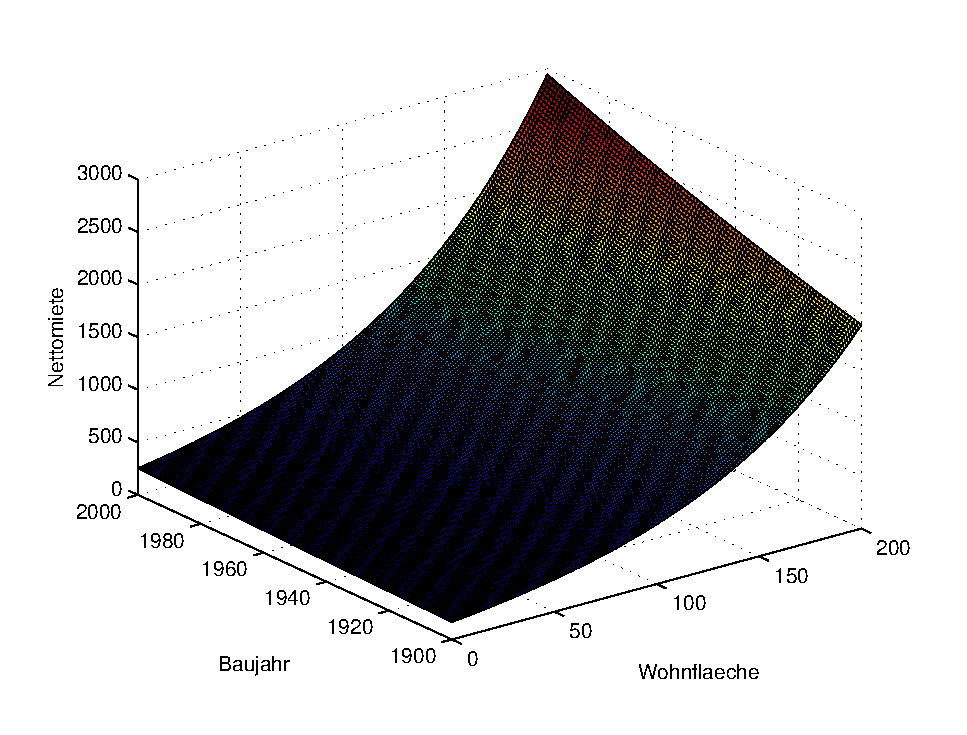
\includegraphics[width=10cm]{figures/nm_wfl_bj_log_approach.eps}
  \end{figure}

\end{frame}

\subsection{Planänderungen}
\begin{frame}
  \frametitle{Regression: Planänderungen}

  \begin{itemize}
  \item Geplant:
    \begin{itemize}
    \item Einfache Regression
    \item Multiple Regression
    \item {\color<2->[gray]{0.4}Robuste Regression (optional)}
    \item Modellauswahl
    \item {\color<2->[gray]{0.4}Modellvalidierung}
    \item Leistungsanalyse
    \end{itemize}
    
    \pause\pause
  
  \item Grund: Platz!
  \end{itemize}

\end{frame}

\section{Anwendung}

\begin{frame}[fragile]
  \frametitle{Anwendung: Testprogramm}
	
	\begin{columns}
		\column{.60\textwidth}
			\begin{lstlisting}
				#include <iostream>
				#include <nag.h>
				#include <nag_stdlib.h>
				#include <nagg02.h>
				
				#include "Timer.h"
				#include "utils.h"
				
				using namespace std;
				
				int main(int argc, char* argv[]) {
	
				  Timer timer;
				
				  int iterations = 100;
				  bool read_file = false;
				  string file_name = "";
				  int size_m = 2;
				  int size_n = 10;
				  bool output_ms = false;
				  bool output_us = false;
				  bool verbose = true;
					
					
					...
			\end{lstlisting}
		\column{.30\textwidth}
			\begin{lstlisting}
								
				// nag-bibliothek
				
				
				
				// eigene klassen/
				// funktionen
				
				
				
								
				
				// timer fuer tests
				
				// eigene argumente
				
				
				
				
				
				
				
				
				
				...
			\end{lstlisting}
	\end{columns}
\end{frame}

\begin{frame}[fragile]
  \frametitle{Anwendung: Testprogramm}
	
	\begin{columns}
		\column{.60\textwidth}
			\begin{lstlisting}
				parse_arguments(argc, argv,
				&iterations, &read_file,
				&file_name, &size_m, &size_n,
				&output_ms, &output_us, &verbose);
				
				Integer n = size_n;
				Integer m = size_m;
				Integer tdx = m;
				double *x = NAG_ALLOC(n * tdx, double);
				Integer *sx = (Integer *)0;
				double *wt = (double *)0;
				Integer tdr = m;
				Integer tdv = m;
				
				double sw;
				double *wmean = NAG_ALLOC(m, double);
				double *std = NAG_ALLOC(m, double);
				double *r = NAG_ALLOC(m * tdr, double);
				double *v = NAG_ALLOC(m * tdv, double);
				NagError fail;
				INIT_FAIL(fail);
				
				
				
				...
			\end{lstlisting}
		\column{.30\textwidth}
			\begin{lstlisting}
				// kommandozeilen-
				// argumente parsen
				
				
				
				// nag-funktion
				// eingabeparameter
				
				
				
				
				
				
				
				// nag-funktion
				// ausgabeparameter
				
				
				
				
				
				
				
				
				...
			\end{lstlisting}
	\end{columns}
\end{frame}

\begin{frame}[fragile]
  \frametitle{Anwendung: Testprogramm}
	
	\begin{columns}
		\column{.60\textwidth}
			\begin{lstlisting}
				if(read_file) {
				  read_matrix_from_file(x, file_name,
				    size_m, size_n, true);
				} else {
				  create_random_matrix(x, size_m, size_n);
				}
				
				if(verbose) {
				  cout << "Starte Leistungstest fuer
				    nag_corr_cov()..." << endl;
				  cout << "Iterationen: " <<
				    iterations << endl;
				}
				
				timer.start();
				
				for(int i = 1; i <= iterations; i++) {
				  nag_corr_cov(n, m, x, tdx, sx, wt, &sw,
				    wmean, std, r, tdr, v, tdv, &fail);
				}
				
				timer.stop();
				
				
				...
			\end{lstlisting}
		\column{.30\textwidth}
			\begin{lstlisting}
				
				// matrix aus datei
				
				
				// matrix per zufall
				
				
				// testausgabe
				
				
				
				
				
				
				// timer starten
				
				
				// nag-funktion
				// anwenden
				
				
				// timer stoppen
				
				
				...
			\end{lstlisting}
	\end{columns}
\end{frame}

\begin{frame}[fragile]
  \frametitle{Anwendung: Testprogramm}
	
	\begin{columns}
		\column{.60\textwidth}
			\begin{lstlisting}
				  if(verbose) {
				    cout << "Korrelationsmatrix:" << endl;
					
				    for(int i = 0; i < m; i++) {
				      for(int j = 0; j < m; j++) {
				        cout << "\t" << R(i, j);
				      }
				      cout << endl;
				    }
				  }
				
				  if(output_ms) {
				    cout << timer.getTimeString_ms() << endl;
				  } else if(output_us) {
				    cout << timer.getTimeString_us() << endl;    
				  } else {
				    cout << timer.getTimeString() << endl;
				  }
				
				  return(0);
				
				}
				
				
				...
			\end{lstlisting}
		\column{.30\textwidth}
			\begin{lstlisting}
				// korrelationsmatrix
				// ausgeben
				
				
				
				
				
				
				
				
				
				// berechnungszeit
				// ausgeben
				
				
				
				
				
				
				
				
				
				
				
				...
			\end{lstlisting}
	\end{columns}
\end{frame}

\section{Leistungsanalyse}

\begin{frame}
  \frametitle{Leistungsanalyse: Testrahmen}
  
  \begin{block}{Verwendetes System (Rechner-Cluster RWTH Aachen)}
  	System: Sun Fire X4450\\
		\begin{itemize}
			\item Anzahl Teilsysteme: 9\\
			\item Architektur: x64\\
			\item Betriebssystem: Linux (CentOS 5.6)\\
			\item Prozessortyp: Xeon X7450 (6 x 2,66 GHz)\\
			\item Anzahl Prozessoren/Kerne pro Teilsystem: 4/24 (insg. 36/216)\\
			\item Arbeitsspeicher: 128 GByte
		\end{itemize}
  \end{block}
  
  \begin{itemize}
		\item Testprogramme nicht parallel programmiert
  \end{itemize}
\end{frame}

\begin{frame}
  \frametitle{Leistungsanalyse: Testrahmen}
  
  \begin{block}{Verwendeter Compiler}
  	Intel C++ 64 Compiler (ICC) 11.1
		\begin{itemize}
			\item standardmäßig Optimierungsstufe O2 aktiviert, um Vergleichbarkeit der einzelnen Tests zu gewährleisten
			\item keine individuellen Optionen gesetzt
		\end{itemize}
  \end{block}
  
  \begin{itemize}
  	\item auf automatische Parallelisierung verzichtet
  \end{itemize}
\end{frame}

\subsection{GNU Scientific Library (GSL)}

\begin{frame}
  \frametitle{GNU Scientific Library (GSL)}
  
  \begin{itemize}
  	\item numerische Bibliothek für C und C++
		\item freie Software unter der {\it GNU General Public License} ({\it GPL})
		\item bietet insgesamt über 1000 Funktionen, darunter auch zahlreiche für statistische Berechnungen
		\item weitere freie Erweiterungen und Wrapper für andere Programmiersprachen ({\it Fortran}, {\it Perl}, {\it Python} etc.) erhältlich
		\item unter anderem von {\it PSPP} genutzt, einer freien Alternative zur professionellen Statistik-Software {\it PASW Statistics} (früher {\it SPSS Statistics})
		\item neben {\it NAG C Library} auf dem Rechner-Cluster verfügbar
  \end{itemize}
\end{frame}

\subsection{Korrelation}

\begin{frame}
	\frametitle{Korrelation: Funktionsübersicht}
	
	\begin{columns}
		\column{.45\textwidth}
			\begin{block}{NAG-Funktionen}
				nag\_corr\_cov\\
				nag\_ken\_spe\_corr\_coeff\\
				nag\_partial\_corr\\
				nag\_sum\_sqs\\
				nag\_sum\_sqs\_update\\
				nag\_cov\_to\_corr\\
				nag\_nearest\_correlation\\
				nag\_robust\_corr\_estim\\
				nag\_robust\_m\_corr\_user\_fn\\
				nag\_robust\_m\_corr\_user\_fn\_no\_derr
			\end{block}
		\column{.45\textwidth}
			\begin{block}{GSL-Funktionen}
				gsl\_stats\_correlation\\
				gsl\_stats\_covariance\\
				gsl\_stats\_covariance\_m
			\end{block}
			\begin{itemize}
				\item weitere Funktionen müssen selbst "`gebastelt"' werden
			\end{itemize}
	\end{columns}
	
	\begin{itemize}
		\item im Bereich Korrelation stellt die NAG-Bibliothek wesentlich mehr fertige Funktionen zur Verfügung
  \end{itemize}
\end{frame}

\begin{frame}
	\frametitle{Korrelation: Vergleich NAG vs. GSL}
	
	Unterschiedliche Ausgaben der Funktionen:

	\begin{block}{nag\_corr\_cov}
		\begin{itemize}
			\item Zwischenberechnungen: arithmetische Mittelwerte, Standardabweichungen und Kovarianzmatrix für alle Merkmale
			\item Korrelationsmatrix mit Bravais-Pearson-Korrelationskoeffizienten für zwei oder mehr Merkmale
		\end{itemize}
	\end{block}
	
	\begin{block}{gsl\_stats\_correlation}
		\begin{itemize}
			\item Bravais-Pearson-Korrelationskoeffizient für genau zwei Merkmale
		\end{itemize}
	\end{block}
	
	\begin{itemize}
			\item für Zwischenberechnungen bietet die GSL-Bibliothek andere Funktionen an, für eine Korrelationsmatrix allerdings nicht
		\end{itemize}
\end{frame}

\begin{frame}
	\frametitle{Korrelation: Testaufbau}
	
	\begin{block}{Testbedingungen}
		\begin{itemize}
			\item Anzahl Iterationen: 1000 pro Schritt
			\item Anzahl Beobachtungen: variabel (10 bis 2050/10000) mit Schrittweite 10
			\item Datensätze:
			\begin{itemize}
				\item {\it Münchener Mietspiegel 2003} (2054 Beobachtungen)
				\item Zufallsdatensatz (10000 Beobachtungen)
			\end{itemize}
		\end{itemize}
	\end{block}
	
	\begin{block}{Tests}
		\begin{itemize}
			\item nag\_corr\_cov vs. gsl\_stats\_correlation
			\item nag\_corr\_cov vs. nag\_ken\_spe\_corr\_coeff
		\end{itemize}
	\end{block}
\end{frame}

\begin{frame}
	\frametitle{Korrelation: Test I}
	
	Mietdatensatz:
	
	\begin{figure}[t]
    \centering
    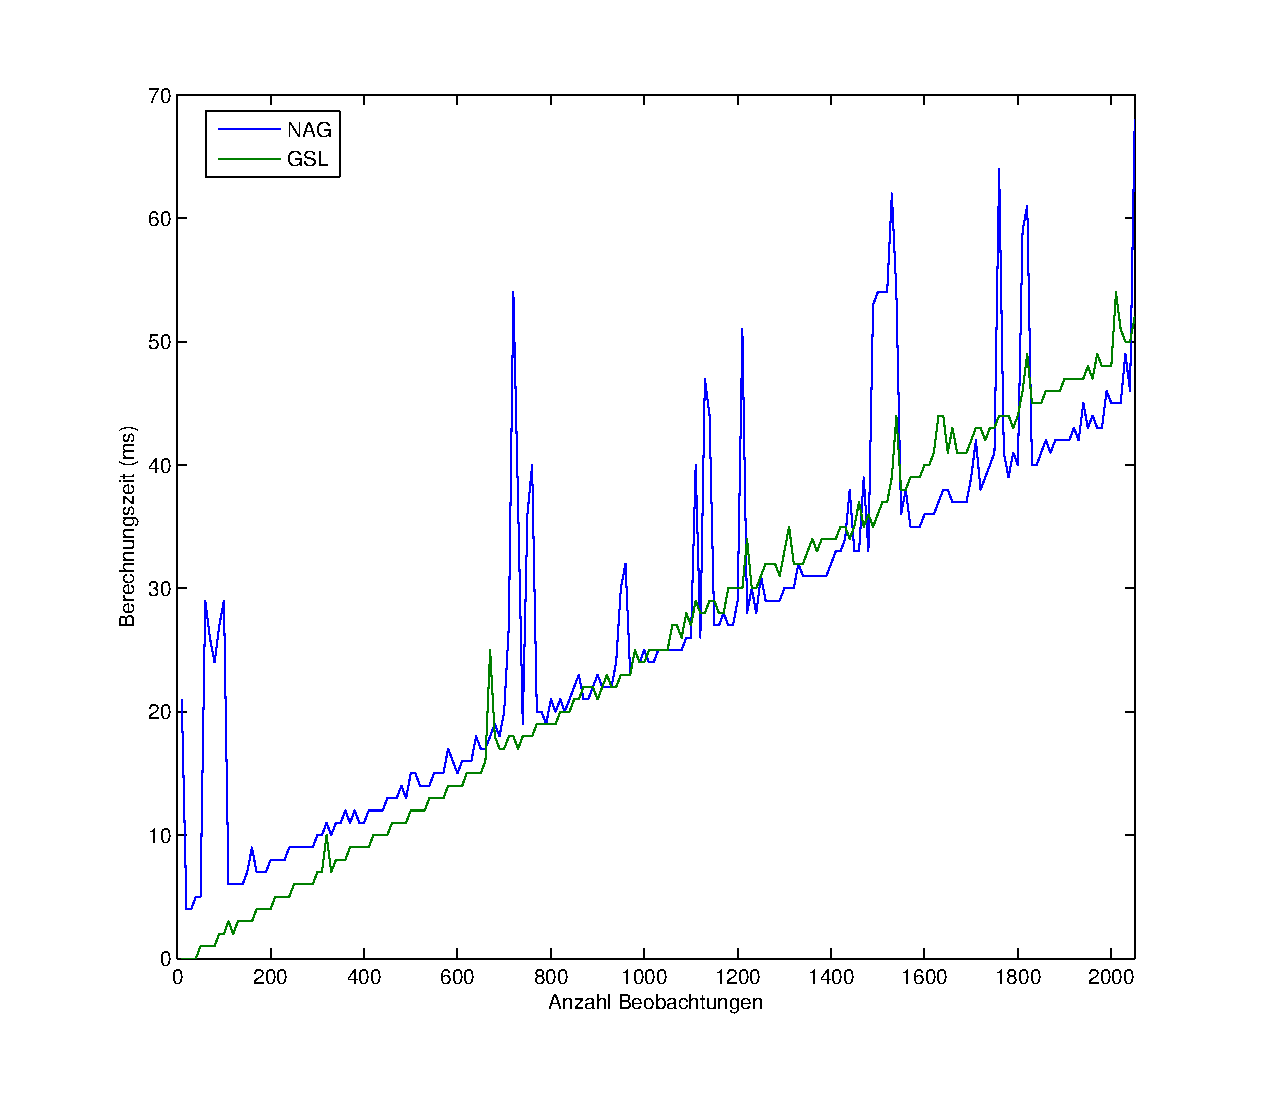
\includegraphics[width=9cm]{figures/test_corr_1_rent.eps}
  \end{figure}
\end{frame}

\begin{frame}
	\frametitle{Korrelation: Test I}
	
	Zufallsdatensatz:
	
	\begin{figure}[t]
    \centering
    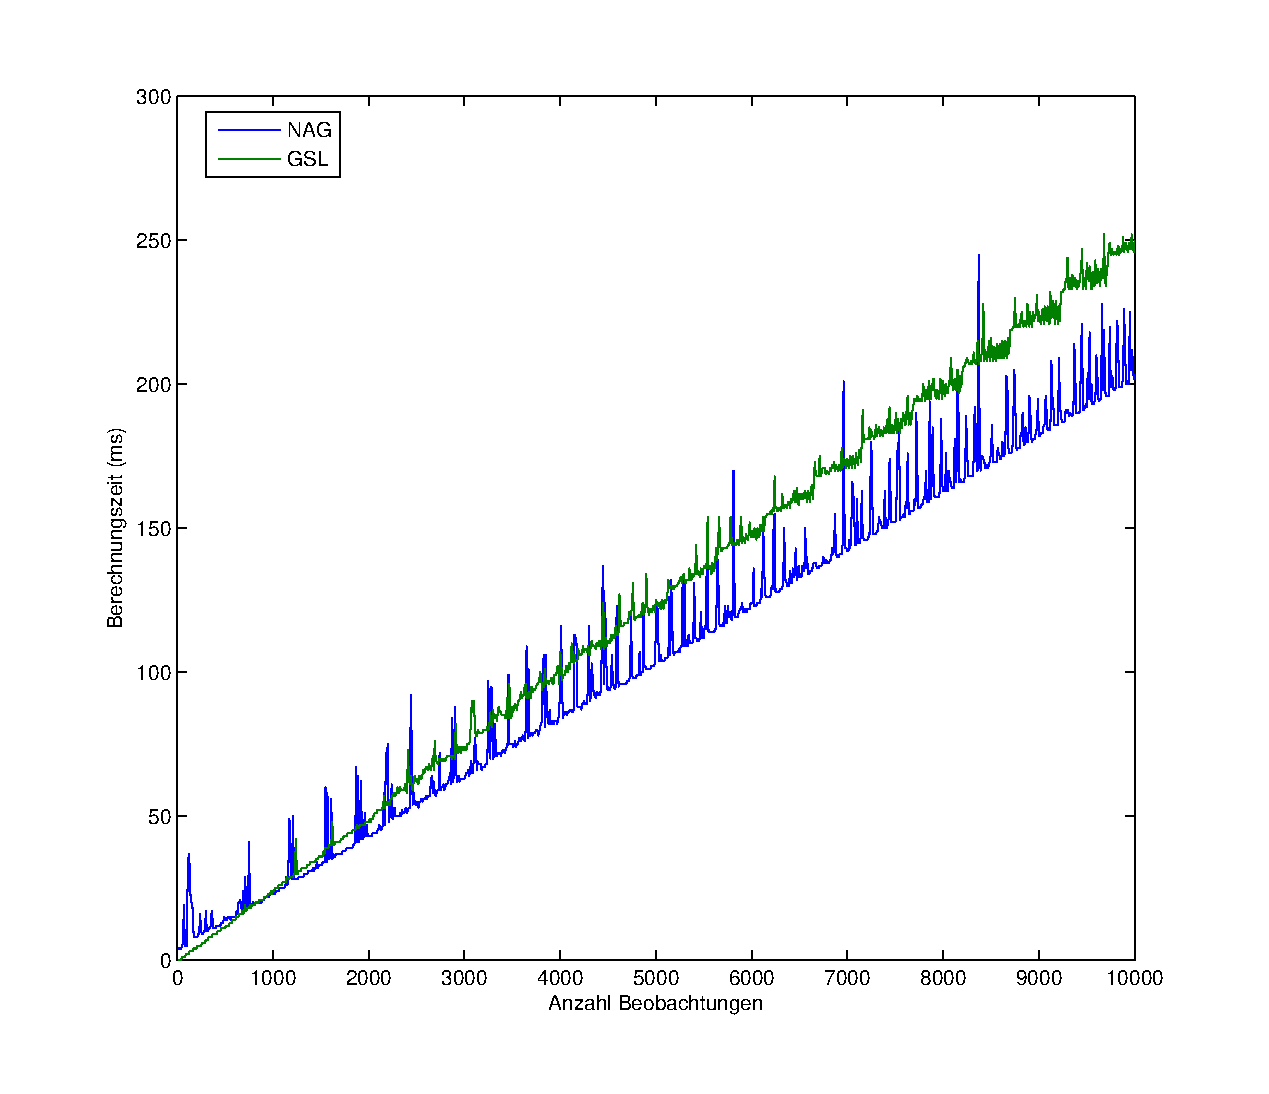
\includegraphics[width=9cm]{figures/test_corr_1_random.eps}
  \end{figure}
\end{frame}

\begin{frame}
	\frametitle{Korrelation: Test II}
	
	Mietdatensatz:
	
	\begin{figure}[t]
    \centering
    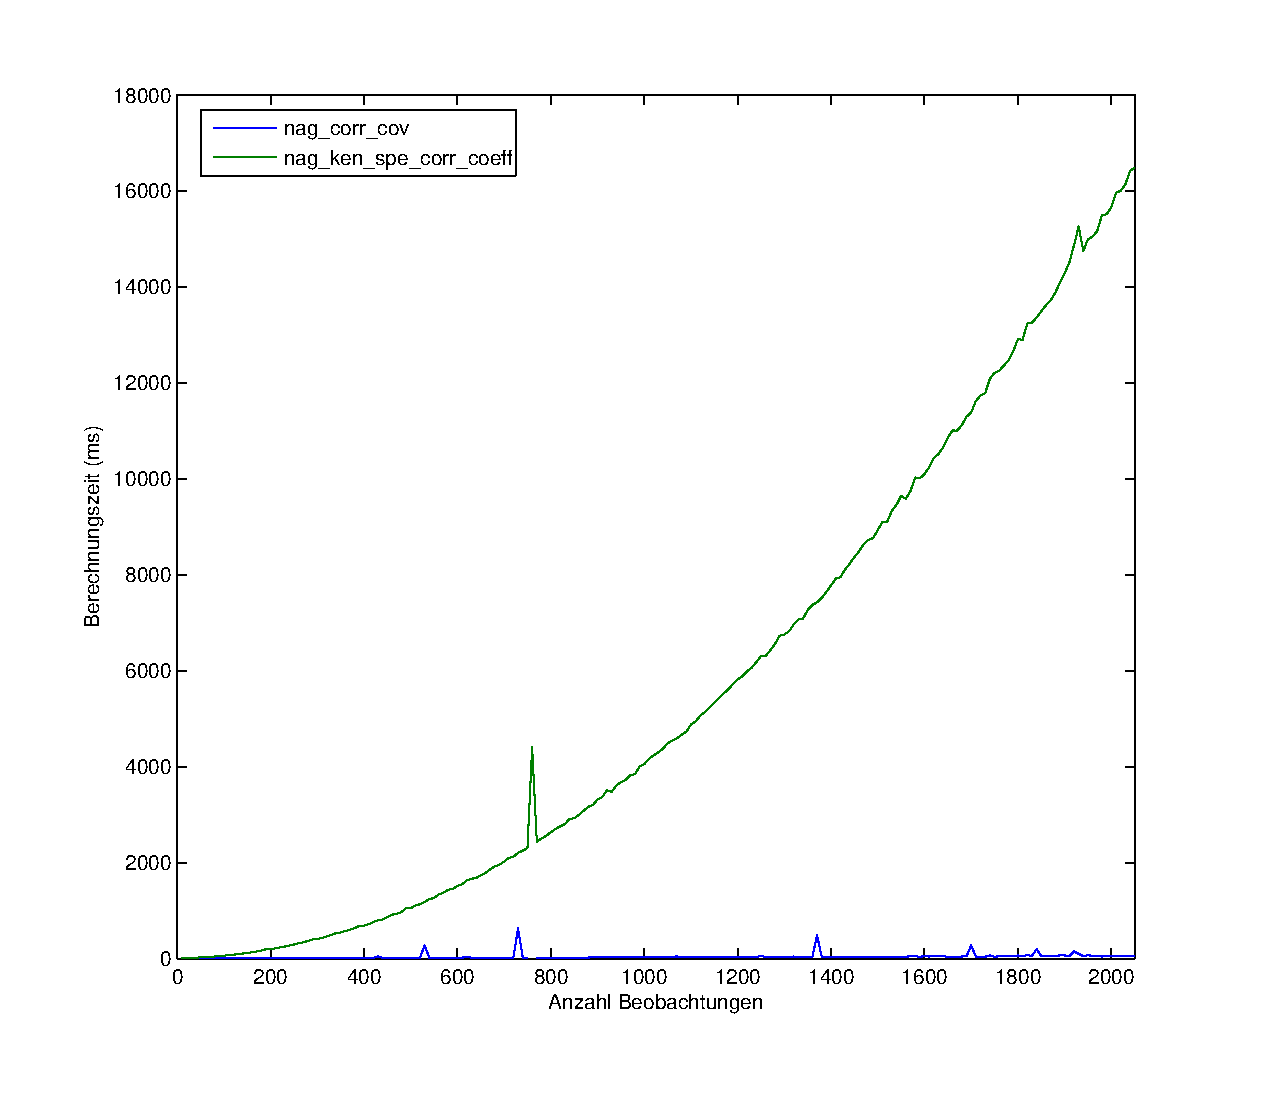
\includegraphics[width=9cm]{figures/test_corr_2_rent.eps}
  \end{figure}
\end{frame}

\begin{frame}
	\frametitle{Korrelation: Test II}
	
	Zufallsdatensatz:
	
	\begin{figure}[t]
    \centering
    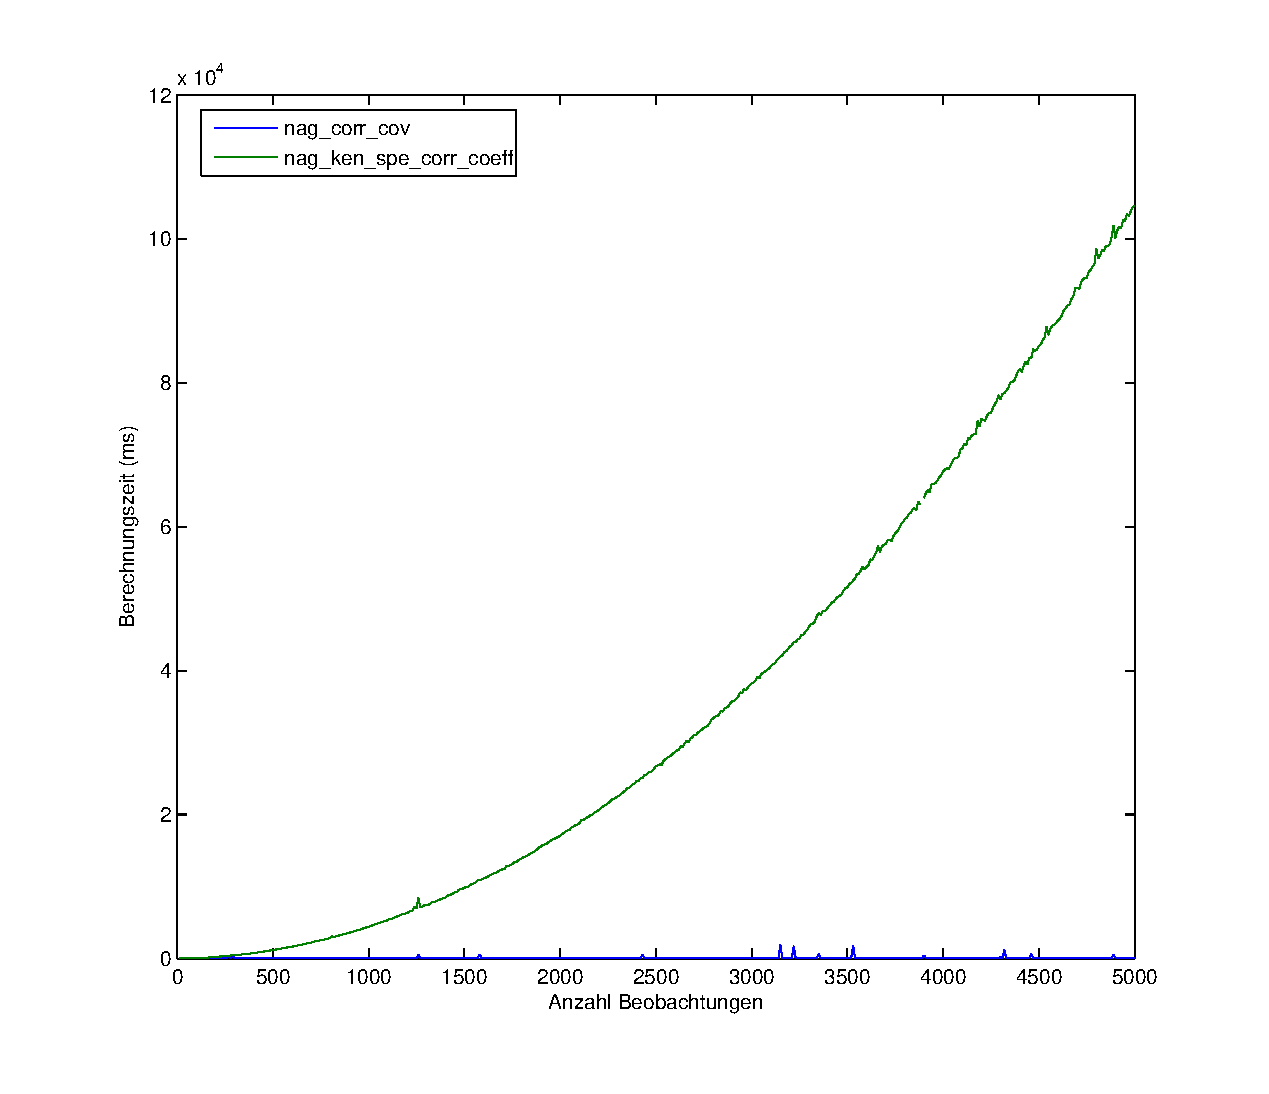
\includegraphics[width=9cm]{figures/test_corr_2_random.eps}
  \end{figure}
\end{frame}

\subsection{Regression}
\begin{frame}
  \frametitle{Regression: Funktionsübersicht}
  
  \begin{columns}
    \column{.45\textwidth}
    \begin{block}{GSL Funktionen}
      \alert<1>{
        gsl\_fit\_linear\\
        gsl\_fit\_wlinear\\
        gsl\_fit\_linear\_est\\
        gsl\_fit\_mul\\
        gsl\_fit\_wmul\\
        gsl\_fit\_mul\_est\\
      }
      \only<2->{\alert<2>{
          gsl\_multifit\_linear\\
          gsl\_multifit\_wlinear\\
          gsl\_multifit\_linear\_svd\\
          gsl\_multifit\_linear\_usvd\\
          gsl\_multifit\_linear\_est\\
          gsl\_multifit\_linear\_residuals\\
        }}
    \end{block}
    \column{.45\textwidth}
    \begin{block}{NAG Funktionen}
      \alert<1>{
        nag\_simple\_linear\_regression\\
      }
      \only<2->{\alert<2>{
          nag\_regsn\_mult\_linear\\
          nag\_regsn\_mult\_linear\_est\_func\\
          nag\_regress\_confid\_interval\\
        }}
      \only<3->{\alert<3>{
          nag\_regsn\_mult\_linear\_addrem\_obs\\
          nag\_regsn\_mult\_linear\_upd\_model\\
          nag\_regsn\_mult\_linear\_add\_var\\
        }}
      \only<4->{\alert<4>{
          nag\_all\_regsn\\
          nag\_step\_regsn\\
        }}
      \only<5->{\alert<5>{
          nag\_glm\_binomial\\
          nag\_glm\_poisson\\
        }}
      \only<6->{\alert<6>{
          nag\_robust\_*\\
          nag\_ridge\_*\\
        }}      
    \end{block}
  \end{columns}

  \pause\pause\pause\pause\pause\pause

  \begin{itemize}
  \item NAG-Bibliothek ist weitaus umfangreicher! 
  \end{itemize}

\end{frame}

\begin{frame}
  \frametitle{Einfache Regression: Vergleich}
  
  \begin{itemize}
  \item Die Funktionen geben unterschiedliche Ergebnisse aus:
  \end{itemize}

  \begin{block}{nag\_simple\_linear\_regression}
    \begin{itemize}
    \item Regressionskoeffizienten
    \item Standardfehler
    \item Quadratsumme der Residuen
    \item Bestimmtheitsmaß $R^2$
    \end{itemize}
  \end{block}

  \begin{block}{gsl\_fit\_linear}
    \begin{itemize}
    \item Regressionskoeffizienten
    \item Kovarianzen
    \item Quadratsumme der Residuen
    \end{itemize}
  \end{block}

\end{frame}

\begin{frame}
  \frametitle{Einfache Regression: Testaufbau}

  \begin{block}{Leistungsanalyse:}
    \begin{itemize}
    \item Iterationen: 1000
    \item Beobachtungen variabel
    \item Unterschiedliche Datensätze:
      \begin{itemize}
      \item Mietdatensatz
      \item Zufällig erzeugte Daten
      \end{itemize}
    \end{itemize}
  \end{block}

\end{frame}

\begin{frame}
  \frametitle{Einfache Regression: Test I} 
  
  \begin{itemize}
  \item Mietdatensatz:
  \end{itemize}

  \begin{figure}[t]
    \centering
    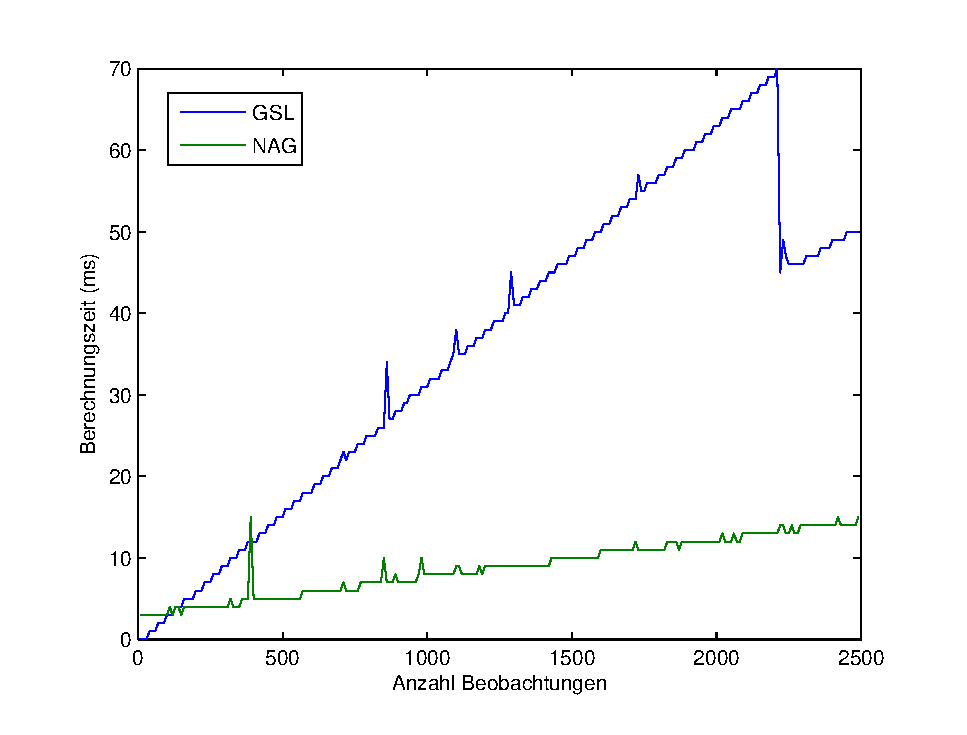
\includegraphics[width=9.5cm]{figures/simple_reg_comp_rent.eps}
  \end{figure}

\end{frame}

\begin{frame}
  \frametitle{Einfache Regression: Test II}

  \begin{itemize}
  \item Zufällige Daten:
  \end{itemize}
  
  \begin{figure}[t]
    \centering
    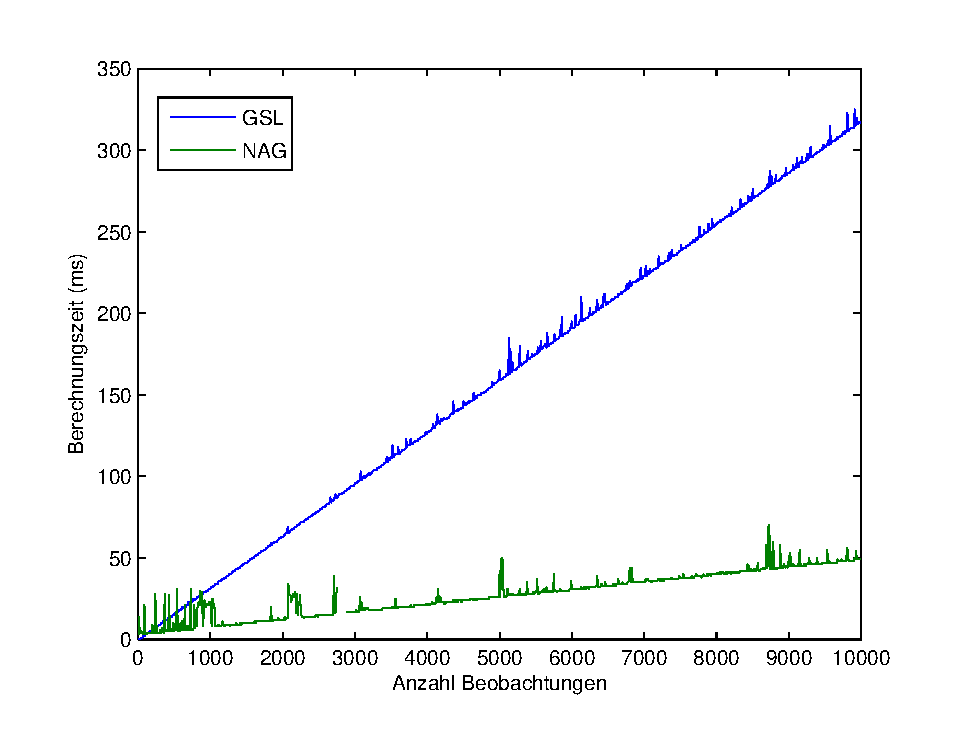
\includegraphics[width=9.5cm]{figures/simple_reg_comp.eps}
  \end{figure}

\end{frame}

\begin{frame}
  \frametitle{Multiple Regression: Vergleich}
  
  \begin{block}{nag\_regsn\_mult\_linear}
    \begin{itemize}
    \item Regressionskoeffizienten
    \item Quadratsumme der Residuen
    \item Standardfehler
    \item Kovarianzmatrix
    \item Residuen
    \item (Zwischenergebnisse)
    \end{itemize}
  \end{block}
  
  \begin{block}{gsl\_multifit\_linear}
    \begin{itemize}
    \item Regressionskoeffizienten
    \item Quadratsumme der Residuen
    \item Kovarianzmatrix
    \end{itemize}
  \end{block}

\end{frame}

\begin{frame}[fragile]
  \frametitle{Multiple Regression: Funktionsaufrufe}
  
  \begin{columns}
    \column{0.5\textwidth}
    \begin{block}{Testprogramm NAG}
      \begin{lstlisting}
timer.start();

for(int i=1; i<=iterations; i++){
  
  nag_regsn_mult_linear(mean, 
    y_size, x, tdx, m, sx, ip, 
    y, wt, &rss, &df, b, se,
    cov, res, h, q, tdq, &svd, 
    &rank, p, tol, com_ar, &fail);

}

timer.stop();
      \end{lstlisting}
    \end{block}
    \column{0.5\textwidth}
    \begin{block}{Testprogramm GSL}
      \begin{lstlisting}
timer.start();

for(int i=1; i<=iterations; i++){    
  
  gsl_multifit_linear(x, y, c, 
    cov, &chisq, wspace);
  
  for(int i=0; i<ip; i++){
    gsl_vector_set(se, i, 
      sqrt(gsl_matrix_get(cov, 
            i, i)));
  }
    
  gsl_multifit_linear_residuals(x, 
    y, c, r);
}

timer.stop();
\end{lstlisting}
\end{block}    
\end{columns}

\end{frame}

\begin{frame}
  \frametitle{Multiple Regression: Testaufbau}
  
  \begin{block}{Test 1:}
    \begin{itemize}
    \item Iterationen: 100
    \item Unabhängige Merkmale: 6
    \item Beobachtungen variabel
    \end{itemize}
  \end{block}

  \begin{block}{Test 2:}
    \begin{itemize}
    \item Iterationen: 100
    \item Beobachtungen: 2500
    \item Unabhängige Merkmale variabel
    \end{itemize}
  \end{block}
  
  \begin{itemize}
  \item Datensätze:
    \begin{itemize}
    \item Mietdatensatz
    \item Zufällig erzeugte Daten
    \end{itemize}
  \end{itemize}
  
\end{frame}

\begin{frame}
  \frametitle{Multiple Regression: Test I}

  \begin{itemize}
  \item Zufällige Daten:
  \end{itemize}

  \begin{figure}[t]
    \centering
    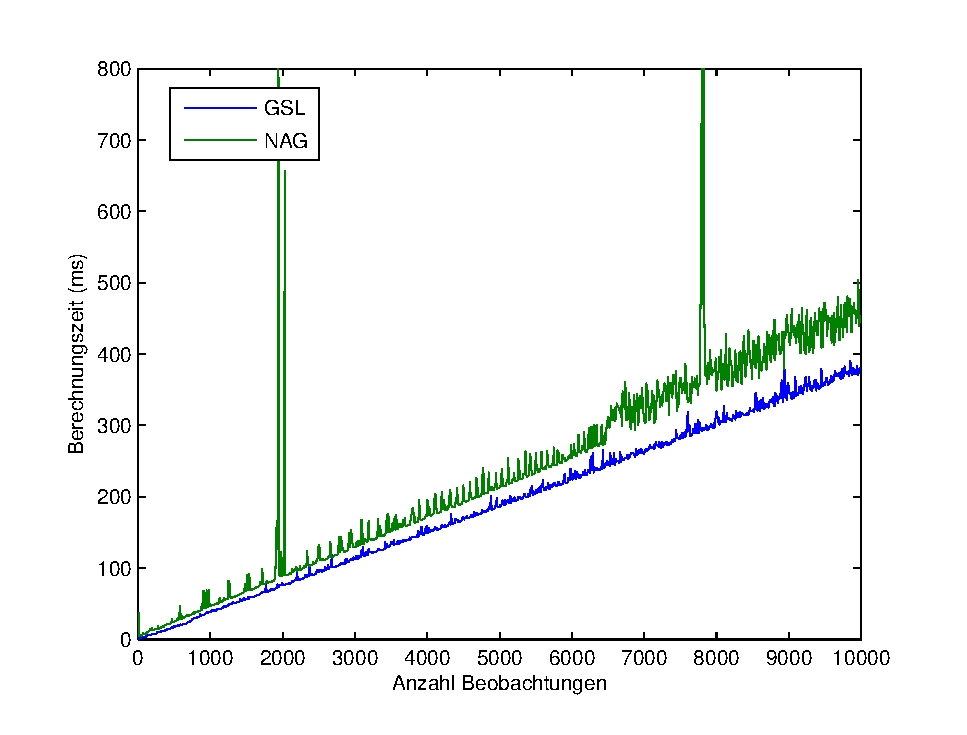
\includegraphics[width=9.5cm]{figures/multi_reg_comp_6_var.eps}
  \end{figure}

\end{frame}

\begin{frame}
  \frametitle{Multiple Regression: Test II}
  \begin{itemize}
  \item Mietdatensatz:
  \end{itemize}

  \begin{figure}[t]
    \centering
    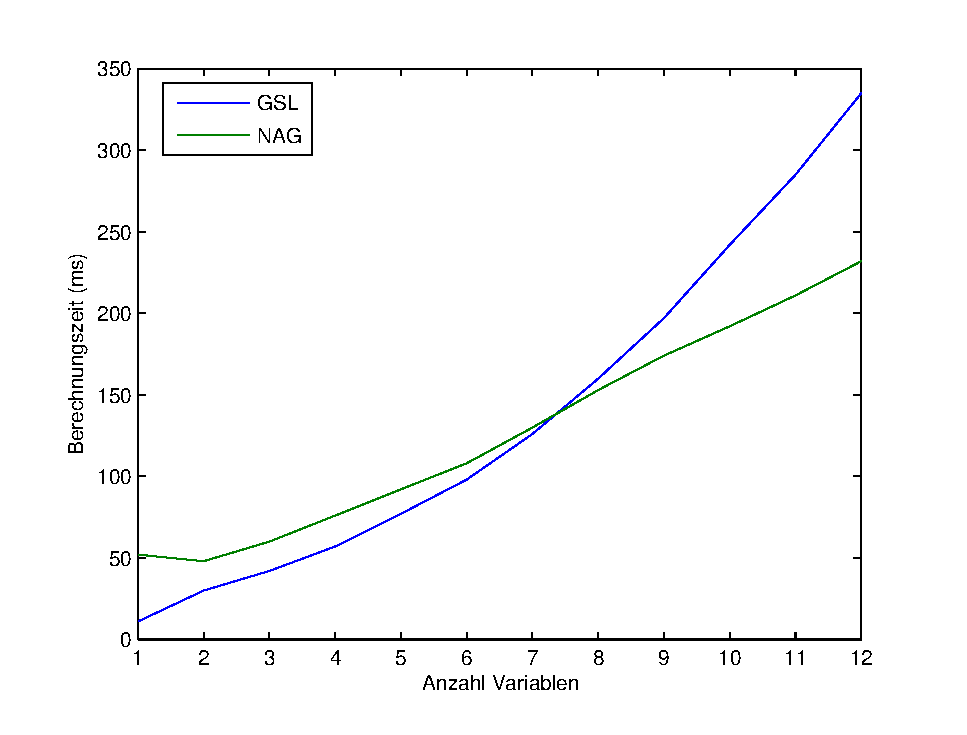
\includegraphics[width=9.5cm]{figures/multi_reg_vars_2500_obs.eps}
  \end{figure}
\end{frame}

\begin{frame}
  \frametitle{Multiple Regression: Test III}
  \begin{itemize}
  \item Zufällige Daten:
  \end{itemize}

  \begin{figure}[t]
    \centering
    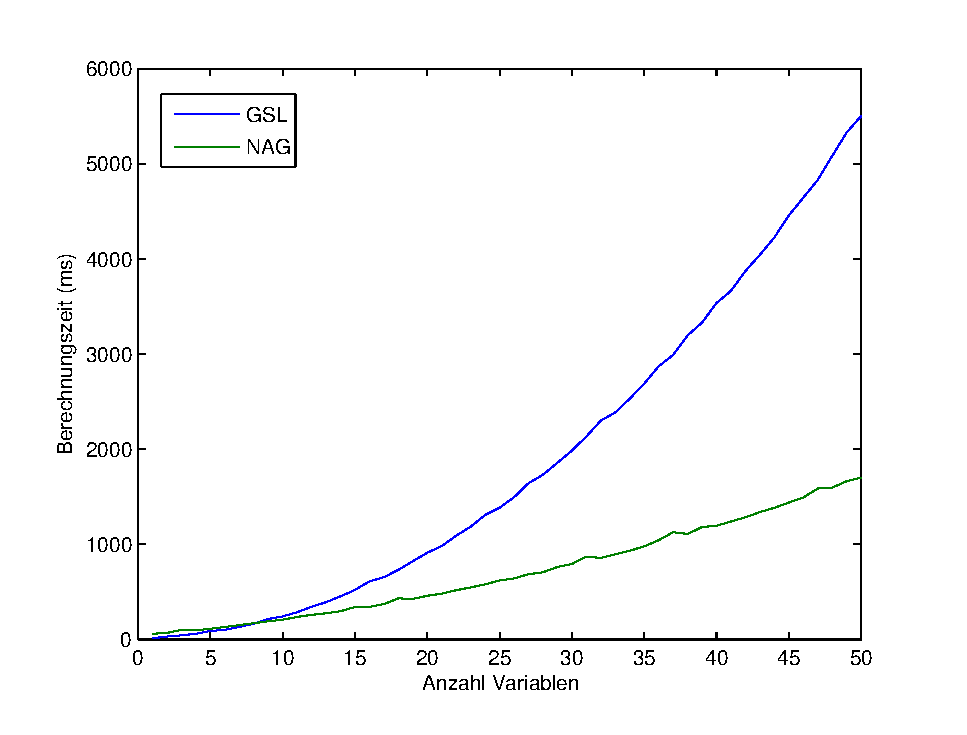
\includegraphics[width=9.5cm]{figures/multi_reg_vars_2500_obs_rand.eps}
  \end{figure}

\end{frame}

\begin{frame}
  \frametitle{Aktualisierung vs. Neuberechnung}
    
  \begin{itemize}
  \item Funktionen zum Aktualisieren des Modells:
    \begin{itemize}
    \item nag\_regsn\_mult\_linear\_addrem\_obs
    \item \alert<3>{nag\_regsn\_mult\_linear\_add\_var}
    \item nag\_regsn\_mult\_linear\_delete\_var
    \item nag\_regsn\_mult\_linear\_addrem\_obs
    \item \alert<3>{nag\_regsn\_mult\_linear\_update\_model}
    \end{itemize}
  \end{itemize}

  \pause

  \begin{itemize}
  \item Wie ändert sich die Performance mit diesen Funktionen?
  \end{itemize}

  \pause

  \begin{itemize}
  \item Testparameter:
    \begin{itemize}
    \item Iterationen: 100
    \item Bobachtungen 2500
    \end{itemize}
  \end{itemize}

\end{frame}

\begin{frame}
  \frametitle{Aktualisierung: Test I}
  
  \begin{itemize}
  \item Mietdatensatz:
  \end{itemize}

  \begin{figure}[t]
    \centering
    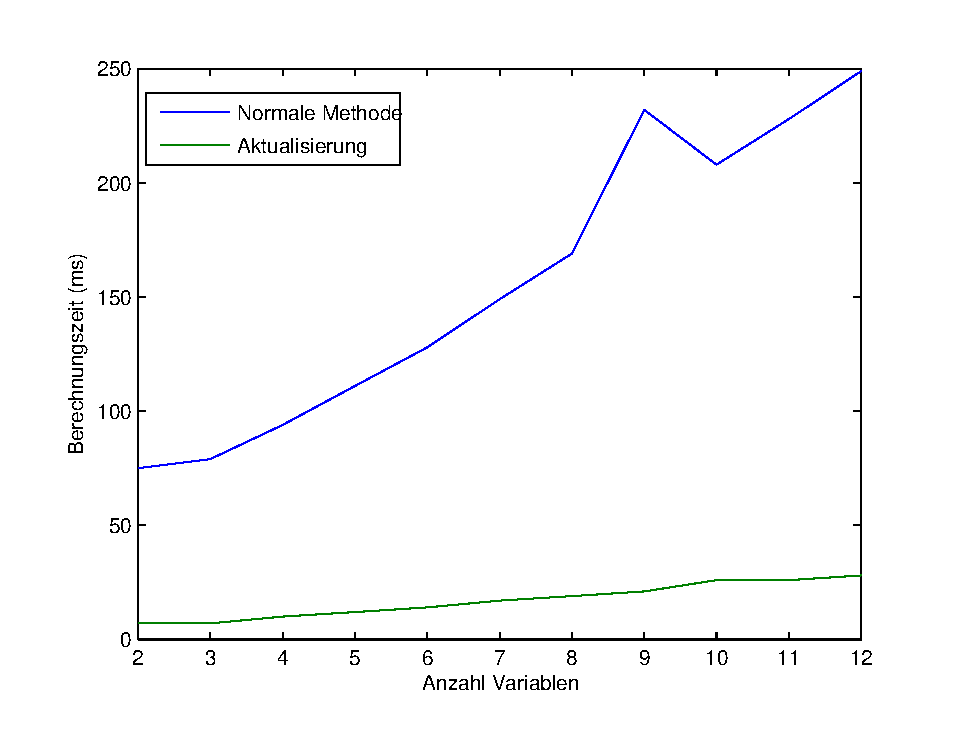
\includegraphics[width=9.5cm]{figures/multi_reg_vars_2500_obs_act.eps}
  \end{figure}

\end{frame}

\begin{frame}
  \frametitle{Aktualisierung: Test II}
  
  \begin{itemize}
  \item Zufällige Daten:
  \end{itemize}

  \begin{figure}[t]
    \centering
    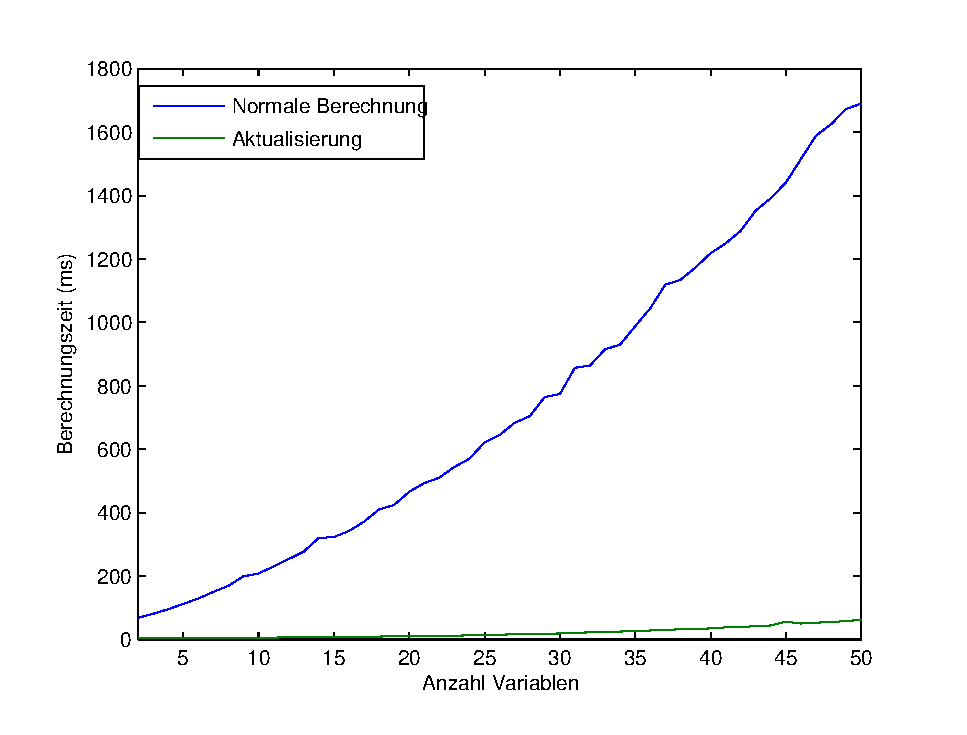
\includegraphics[width=9.5cm]{figures/multi_reg_vars_2500_obs_act_rand.eps}
  \end{figure}

\end{frame}


\section{Fazit}
\begin{frame}
  \frametitle{Fazit}
  
  \begin{itemize}
  \item NAG Bibliothek für Korrelation und Regression gut geeignet
  \item Im Vergleich zur GSL:
    \begin{itemize}
    \item (Meist) effizientere Implementierung
    \item Größerer Funktionsumfang
    \item Zusätzliche Hilfsfunktionen (z.B. nag\_step\_regsn)
    \item Funktionen werden umfangreich getestet
    \end{itemize}
  \end{itemize}
  
\end{frame}

\begin{frame}
  \frametitle{}

  \begin{center}
    {\Large Vielen Dank für die Aufmerksamkeit!}
  \end{center}

\end{frame}

\end{document}
